\documentclass{article}

\usepackage{iclr2027_conference,times}
\usepackage{amsmath}
\usepackage{amssymb}
\usepackage{amsthm}
\usepackage{booktabs}
\usepackage{graphicx}
\usepackage{microtype}
\usepackage{url}
\usepackage{enumitem}

\title{The Inference Value Theorem: Exact Finite-Sample Laws for Best-of-N Selection}

\author{Anonymous Authors}

\newtheorem{theorem}{Theorem}
\newtheorem{corollary}{Corollary}
\newcommand{\acc}{\mathrm{acc}}
\newcommand{\ind}{\mathbf{1}}
\newcommand{\E}{\mathbb{E}}
\newcommand{\Kappa}{\kappa}

\begin{document}

\maketitle

\begin{abstract}
Best-of-$N$ sampling is a standard way to improve language-model accuracy:
generate multiple candidate responses, score them, and return the highest
scoring candidate. Its behavior is often summarized by pairwise score metrics
such as AUC, but pairwise separation does not determine high-$N$ performance.
We derive an exact finite empirical law for best-of-$N$ selection under any
scalar score with random tie-breaking. The law shows that expected
best-of-$N$ accuracy is governed by the conditional score-rank moment
structure; AUC/kappa is the complete special case only for $N=2$. We validate
the law across a 23-model theorem-aligned bundle, where the exact-law
prediction attains mean absolute error (MAE) $6.22\times 10^{-4}$ and the
moment predictor is exact up to $7.44\times 10^{-18}$. We further report
finite-pilot forecasting, learned-verifier and live-judge scores, four
pilot-scale cross-benchmark families, adaptive allocation, and a scoped
119-record 4096-sample held-out MATH slice. The evidence supports the
theorem's empirical relevance while explicitly leaving manifest-scale
held-out coverage, six-family benchmark coverage, and broad live-judge
generality as future work.
\end{abstract}

\section{Introduction}

Best-of-$N$ inference converts additional sampling into accuracy by selecting
one response from a set of candidates. The same template underlies verifier
reranking, reward-model selection, LLM-as-a-judge scoring, and likelihood
reranking \citep{cobbe2021training,zheng2023judging}. The practical question
is not only whether a score is better than random pairwise ranking. It is how
that score changes the entire best-of-$N$ curve as $N$ grows.

The common pairwise answer is AUC. AUC is meaningful: for best-of-two
selection, it is exactly the right summary once the base correctness rate is
known. For $N>2$, however, it discards where correct responses lie in the
score-rank distribution. Two scorers can have the same pairwise AUC and
different high-$N$ behavior if one places a few correct responses at the very
top while the other spreads correct responses through the middle ranks.

This paper gives a finite-sample answer. For any fixed problem, finite
response pool, scalar score, and random tie-breaking rule, expected
best-of-$N$ accuracy is an exact order-statistic functional of the empirical
score-label distribution. The formula is not asymptotic and does not assume a
particular score family. It applies equally to log probability, learned
verifier scores, calibrated posteriors, live judge scores, heuristic scores,
and oracle diagnostic scores.

The empirical contribution is deliberately scoped. We validate the theorem and
its moment hierarchy across 23 models, then test whether the same law is
useful for finite-pilot forecasting, verifier-style reranking, live judge
scores, cross-benchmark pilots, and adaptive allocation. We do not claim that
the current artifacts complete a full maxed-out manifest. The strongest
supported claim is theorem-first: best-of-$N$ evaluation should report the
score-rank moment structure, not only AUC.

\paragraph{Contributions.}
We make four contributions. (1) We derive an exact finite empirical selector
law for best-of-$N$ selection with arbitrary scalar scores and random
tie-breaking. (2) We show that AUC/kappa is complete for $N=2$ and
insufficient for higher $N$, where rank-interval moments are necessary.
(3) We validate the law on a 23-model theorem-aligned bundle with exact-law
MAE $0.000622$ and moment-hierarchy error at floating-point scale. (4) We
report scoped evidence for finite pilots, learned and live judge scores,
cross-benchmark task broadening, adaptive allocation, and a 119-record
4096-depth held-out MATH slice, while separating passed gates from missing
manifest-scale gates.

\section{Setup}

Fix one problem and a finite empirical response pool of size $n$. Response
$i$ has correctness label $Y_i\in\{0,1\}$ and scalar score $S_i$. Let
$p=n^{-1}\sum_i Y_i$ be the empirical base correctness rate. Best-of-$N$
draws $N$ candidates independently with replacement from the empirical pool
and returns a response with maximum score, breaking top-score ties uniformly
at random. Let $f_N$ denote the expected correctness of the selected response.

Sampling with replacement matches the experiment simulator and the usual
interpretation of the empirical pool as a finite distribution over candidate
draws. The same rank formula can be adapted to without-replacement sampling,
but that is not the protocol evaluated here.

\section{Exact Selector Law}

Sort responses by nondecreasing score. For each tied score group $g$, let
$[a_g,b_g]$ be its one-indexed rank interval, $k_g=b_g-a_g+1$ its size, and
$c_g=\sum_{i\in g}Y_i$ the number of correct responses in the group.

\begin{theorem}[Finite empirical best-of-$N$ law]
\label{thm:selector}
Under the empirical with-replacement protocol above and uniform random
tie-breaking among top-score ties,
\begin{equation}
\label{eq:selector-law}
f_N =
\sum_g \frac{c_g}{k_g}
\left[
\left(\frac{b_g}{n}\right)^N
-
\left(\frac{a_g-1}{n}\right)^N
\right].
\end{equation}
For $N=1$, this reduces to $f_1=p$.
\end{theorem}

The bracketed term is the probability that the maximum rank among the $N$
draws falls inside tied group $g$; the factor $c_g/k_g$ is the expected
correctness after uniform tie-breaking within that group. The proof is a
one-line partition of the maximum-rank event, and is given in
Appendix~\ref{app:proof}.

\paragraph{Moment view.}
When $p>0$, define the empirical rank-interval moment
\begin{equation}
\theta_{N-1}=\frac{f_N}{Np}.
\end{equation}
Then $f_N=Np\theta_{N-1}$. In the continuous no-tie limit,
$\theta_{N-1}$ is the $(N-1)$st moment of the mixture CDF evaluated at a
correct response's score. The finite interval form in
Equation~\ref{eq:selector-law} is the exact version used in the experiments.

\paragraph{AUC is the $N=2$ special case.}
Let $\Kappa=\Pr(S^+>S^-)+\tfrac{1}{2}\Pr(S^+=S^-)$ be the Mann-Whitney AUC
with tie handling matched to the selector. For $N=2$,
\begin{equation}
\label{eq:n2}
f_2=p^2+2p(1-p)\Kappa .
\end{equation}
The terms correspond to drawing two correct responses, or drawing one correct
and one incorrect response and selecting the correct one. For $N>2$, AUC is
not sufficient: Equation~\ref{eq:selector-law} depends on higher powers of the
rank intervals, so high-score tail placement matters.

\section{Empirical Protocol}

All results are computed from repository artifacts generated before this
manuscript package. The theorem-aligned experiments evaluate
$N\in\{1,2,4,8,16,32,48\}$ across 23 model directories with up to 500 MATH
records per model \citep{hendrycks2021math}. The primary score is mean log
probability unless otherwise stated. We compare the exact empirical
best-of-$N$ measurement to Equation~\ref{eq:selector-law}.

For finite-pilot experiments, pilot samples estimate the score-rank law and
held-out response pools evaluate predictions. Learned verifiers use
problem-level train/test splits, not response-level leakage. Oracle
correctness and synthetic verifier scores are included only as diagnostic
upper bounds. The live-judge and cross-benchmark experiments are scoped to
completed subsets. A claim-gate report records which ideal gates pass and
which remain missing; no partial raw-cache record is counted as held-out
evidence.

\section{Theorem-Aligned Results}

\begin{table}[t]
\centering
\caption{Core theorem-aligned evidence. The exact law is problem-conditional;
pooling heterogeneous problems destroys the conditional structure.}
\label{tab:core}
\begin{tabular}{l r}
\toprule
Quantity & Value \\
\midrule
Models & 23 \\
Problems per model & up to 500 \\
Exact-law overall MAE & 0.000622 \\
Tie rate & 0.000134 \\
Per-problem MAE & 0.000602 \\
Pooled MAE & 0.122364 \\
\bottomrule
\end{tabular}
\end{table}

Table~\ref{tab:core} shows the main theorem validation. The exact selector law
predicts the measured best-of-$N$ curve with overall MAE $0.000622$ across
35,964 model/problem/$N$ triples. The pooled baseline is much worse because
best-of-$N$ selection depends on the within-problem score-label distribution;
pooling across heterogeneous problems discards that conditioning.

\begin{figure}[t]
\centering
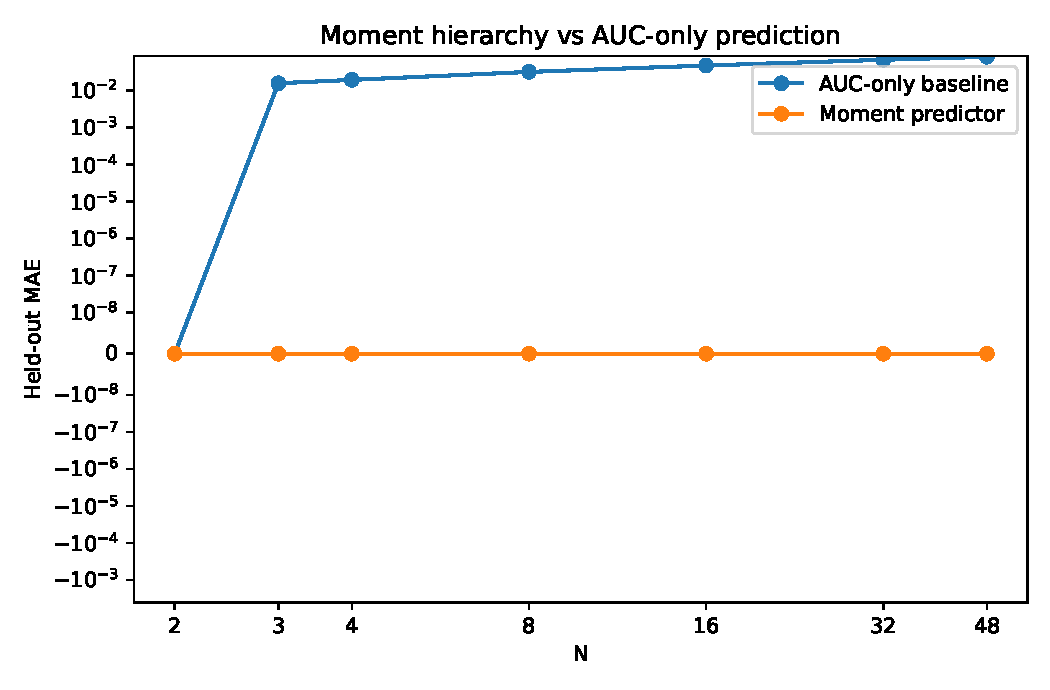
\includegraphics[width=.82\linewidth]{figures/moment_hierarchy_vs_auc.pdf}
\caption{AUC/kappa is exact at $N=2$, but its error grows at high $N$.
The rank-interval moment predictor remains exact up to floating-point error.}
\label{fig:moment}
\end{figure}

Figure~\ref{fig:moment} tests whether pairwise AUC is enough to predict the
curve. It is exact at $N=2$, as Equation~\ref{eq:n2} predicts, but the
AUC-only MAE grows from $0.0158$ at $N=3$ to $0.0821$ at $N=48$. The moment
predictor remains exact up to numerical error, with maximum observed MAE
$7.44\times10^{-18}$. This is the central empirical message: high-$N$
best-of-$N$ evaluation is a moment problem, not a pairwise-summary problem.

\section{Estimation and Scoped Extensions}

\paragraph{Finite pilots.}
The exact law assumes the scored empirical response distribution is known.
The finite-pilot experiments ask how forecasting improves as the pilot size
$K$ increases. The expanded pilot covers five models, 100 stratified MATH
problems per model, 256 samples per problem, 20 seeds, and
$K\in\{8,16,24,32,48,64,96,128,192\}$. For $N=8$, held-out MAE decreases
from $0.093$ at $K=8$ to $0.034$ at $K=128$, with $0.039$ at $K=192$
(Figure~\ref{fig:pilot}). This supports a sample-complexity curve, not a
claim that tiny pilots are universally sufficient.

\begin{figure}[t]
\centering
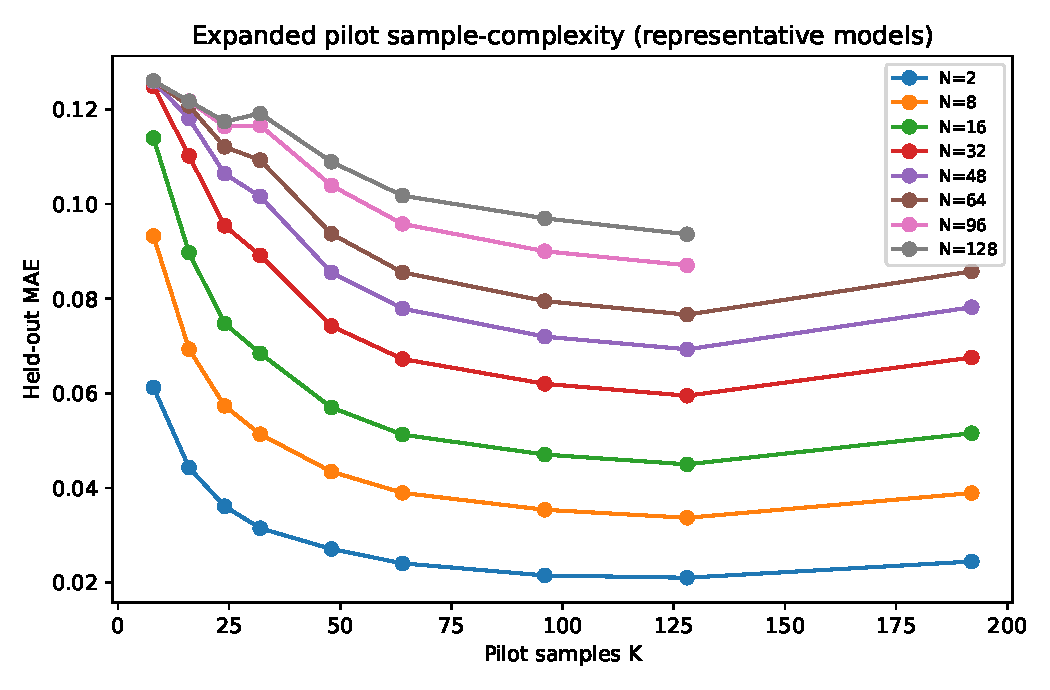
\includegraphics[width=.82\linewidth]{figures/expanded_pilot_sample_complexity.pdf}
\caption{Expanded five-model pilot forecasting. Larger pilots generally
reduce held-out error for $N=8$, but the curve is still sample-limited.}
\label{fig:pilot}
\end{figure}

\paragraph{Held-out 4096-depth slice.}
The maxed-out held-out campaign is incomplete, but it contains 119 contiguous
3B/MATH records, problem 0 through problem 118, each measured at 4096 samples.
On the locked diagnostic row for $K=128/256/512,N=8$, the selected estimator
is \texttt{oracle\_full\_distribution}, with MAE $0.00564$, median absolute
error $0.00356$, maximum absolute error $0.02670$, and 119 rows. This row is
useful as a full-depth diagnostic of the measurement and gate machinery; it is
not presented as a deployable finite-pilot estimator. Problem 119 has only
3152/4096 valid raw-cache samples and is not counted.

\begin{table}[t]
\centering
\caption{Scoped extensions. All rows are paper-facing only at the stated
scale; maximum-scope generality remains limited by missing gates.}
\label{tab:extensions}
\begin{tabular}{p{0.31\linewidth}p{0.28\linewidth}p{0.29\linewidth}}
\toprule
Evidence & Scale & Main result \\
\midrule
Learned verifiers & 5 feature-rich models, problem-level splits &
GBDT AUC 0.8505, $N=48$ accuracy 0.5823 \\
Live judge score & 135/135 model/problem pairs, 6480 judgments &
$N=48$ accuracy 0.5608 vs. 0.4963 for mean logprob \\
Cross-benchmark pilots & GPQA, IFEval, LiveBench, LiveCodeBench; 16 models,
20 tasks, 48 samples & 320/320 records per family; exact-law MAE 0.0 \\
Adaptive allocation & 5-model expanded pilot, fixed budgets &
Moment-law policy improves over uniform by 0.0125 \\
\bottomrule
\end{tabular}
\end{table}

Table~\ref{tab:extensions} summarizes score-agnostic and task-broadening
evidence. Learned feature-based verifiers show that the law applies beyond
likelihood scores. A live LLM judge improves over mean log probability on the
completed 45-problem subset, while remaining governed by the same exact law.
Cross-benchmark pilots cover GPQA Diamond \citep{rein2023gpqa}, IFEval
\citep{zhou2023ifeval}, LiveBench selected \citep{white2024livebench}, and
LiveCodeBench \citep{jain2024livecodebench}, with complete pilot-scale
measurement and exact-law MAE 0.0 in each family. Adaptive allocation is
positive but modest; the oracle policy remains an upper bound rather than an
achieved deployment policy.

\section{Claim Status and Limitations}

\begin{table}[t]
\centering
\caption{Current claim-gate status. Passed gates support scoped wording;
missing gates are explicitly excluded from the main claims.}
\label{tab:gates}
\begin{tabular}{p{0.48\linewidth}p{0.16\linewidth}p{0.23\linewidth}}
\toprule
Claim or gate & Status & Evidence scale \\
\midrule
Core exact-law MAE and moment exactness & PASS & 23-model theorem bundle \\
Held-out $K=128/256/512,N=8$ diagnostic rows & PASS & 119 3B/MATH records \\
Live judge delta over logprob & PASS & 135 completed pairs \\
Cross-benchmark exact-law coverage & PASS & 4 pilot families \\
Adaptive allocation delta & PASS & 5-model pilot \\
Full held-out MATH manifest & MISSING & target 11,500 records \\
Maxed live-judge coverage & MISSING & target at least 8000 pairs \\
Six-family manifest-scale benchmarks & MISSING & missing MATH500 and MBPP-backed family \\
\bottomrule
\end{tabular}
\end{table}

The limitations are central to the paper's claim policy. First, the strongest
held-out evidence is a 119-record 3B/MATH slice, not full 23-model,
500-problem, 4096-depth coverage. Second, the cross-benchmark results are
pilot-scale: four families at 20 tasks and 48 samples per model/task, not six
families at 500 tasks and 128 samples. Third, the live-judge improvement is
scoped to the completed subset and does not establish broad judge
superiority. Fourth, finite-pilot forecasting remains sample-limited. Fifth,
adaptive allocation is directionally useful but not globally optimal.

\section{Conclusion}

Best-of-$N$ selection has an exact finite empirical law. This law explains why
AUC/kappa is exact for $N=2$ but insufficient for larger candidate sets, where
score-rank moment structure controls performance. The current evidence
validates the theorem across a broad theorem-aligned bundle and shows scoped
utility for pilots, verifiers, judges, benchmark broadening, and allocation.
The next empirical step is scale, not a new theorem: complete the missing
manifest gates while preserving the same conditional, rank-based evaluation.

\section*{Reproducibility Statement}
All paper-facing numbers are traceable to artifacts under
\path{results/du_aligned/}, \path{results/benchmarks/}, and
\path{results/maxed_out/}. The exact selector implementation is in
\path{src/theorem.py} and the theorem-aligned runner is
\path{experiments/09_du_aligned.py}. The appendix lists the specific evidence
files and includes the proof of Theorem~\ref{thm:selector}.

\section*{Ethics Statement}
This work analyzes evaluation methodology for language-model inference. It
does not release new human-subject data, alter benchmark ground truth, or
train models for deployment. The main ethical risk is overclaiming from
partial evidence; the paper mitigates this by exposing missing gates and
scoping live-judge and cross-benchmark conclusions to completed artifacts.

\bibliographystyle{iclr2026_conference}
\bibliography{references}

\appendix
\section{Proof}
\label{app:proof}

We prove Theorem~\ref{thm:selector}. Sort the empirical response pool by
nondecreasing score and group identical scores. Let $M$ be the maximum sorted
rank among the $N$ independent draws. For a tied group $g$ occupying ranks
$[a_g,b_g]$,
\[
\Pr(M\in[a_g,b_g])
=
\Pr(M\leq b_g)-\Pr(M\leq a_g-1)
=
\left(\frac{b_g}{n}\right)^N
-
\left(\frac{a_g-1}{n}\right)^N .
\]
Conditioned on $M\in[a_g,b_g]$, all selected top-score candidates lie inside
group $g$. Uniform random tie-breaking makes the selected response correct
with probability $c_g/k_g$. Summing over the disjoint tied-score groups gives
Equation~\ref{eq:selector-law}. For $N=1$, each empirical response is selected
with probability $1/n$, so $f_1=p$.

\section{AUC Special Case}
\label{app:auc}

For $N=2$, draw two empirical responses. With probability $p^2$, both are
correct and the selected response is correct. With probability
$2p(1-p)$, exactly one is correct; conditional on this event, the probability
that the correct response wins the score comparison, including half credit for
ties induced by uniform tie-breaking, is
$\Kappa=\Pr(S^+>S^-)+\frac{1}{2}\Pr(S^+=S^-)$. With probability
$(1-p)^2$, both are incorrect. Therefore
\[
f_2 = p^2 + 2p(1-p)\Kappa .
\]
For $N>2$, events involving the maximum among three or more draws depend on
higher powers of the empirical rank CDF, which is why the scalar pairwise
quantity $\Kappa$ is not generally sufficient.

\section{Additional Result Tables}
\label{app:tables}

\begin{table}[t]
\centering
\caption{Moment hierarchy MAE by $N$ on the response-pool held-out split.}
\label{tab:moment-values}
\begin{tabular}{r r r}
\toprule
$N$ & AUC-only MAE & Moment MAE \\
\midrule
2 & 0.000000 & $7.05\times10^{-18}$ \\
3 & 0.015816 & $4.94\times10^{-18}$ \\
4 & 0.019492 & $7.43\times10^{-18}$ \\
8 & 0.032017 & $6.57\times10^{-18}$ \\
16 & 0.047628 & $7.44\times10^{-18}$ \\
32 & 0.068146 & $6.68\times10^{-18}$ \\
48 & 0.082098 & $4.08\times10^{-18}$ \\
\bottomrule
\end{tabular}
\end{table}

\begin{table}[t]
\centering
\caption{Expanded pilot $N=8$ held-out forecasting MAE. The curve supports
sample-complexity analysis, not tiny-pilot sufficiency.}
\label{tab:pilot-values}
\begin{tabular}{r r}
\toprule
$K$ & Held-out MAE \\
\midrule
8 & 0.093 \\
16 & 0.069 \\
24 & 0.057 \\
32 & 0.051 \\
48 & 0.043 \\
64 & 0.039 \\
96 & 0.035 \\
128 & 0.034 \\
192 & 0.039 \\
\bottomrule
\end{tabular}
\end{table}

\begin{table}[t]
\centering
\caption{Pilot-scale cross-benchmark summary. All four completed families
have complete measured coverage at the requested pilot scale.}
\label{tab:cross-values}
\begin{tabular}{l r r r r}
\toprule
Benchmark & Records & Nondeg. & Law MAE & $N=48$ acc. \\
\midrule
GPQA Diamond & 320/320 & 251 & 0.0 & 0.5890 \\
IFEval & 320/320 & 164 & 0.0 & 0.7962 \\
LiveBench selected & 320/320 & 141 & 0.0 & 0.2546 \\
LiveCodeBench & 320/320 & 262 & 0.0 & 0.5246 \\
\bottomrule
\end{tabular}
\end{table}

\begin{table}[t]
\centering
\caption{Reference-budget adaptive allocation ranking on the expanded-pilot
setting. Oracle is an upper bound, not a deployable policy.}
\label{tab:allocation-values}
\begin{tabular}{l r}
\toprule
Policy & Accuracy \\
\midrule
Oracle & 0.6644 \\
AUC/kappa-based & 0.6359 \\
Moment-law & 0.6351 \\
$p$-based & 0.6255 \\
Uniform & 0.6226 \\
\bottomrule
\end{tabular}
\end{table}

\section{Evidence Manifest}
\label{app:evidence}

The final wording was checked against the following repository artifacts.

\begin{itemize}[leftmargin=*]
\item Core score-rank law and moment hierarchy:
\path{results/du_aligned/du_experiment_results.json} and
\path{results/du_aligned/du_experiment_summary.txt}.
\item Expanded pilots, learned verifiers, live judge scores, and adaptive
allocation:
\path{results/du_aligned/paper_claims_status.md},
\path{results/du_aligned/live_judge_score_summary.json}, and
\path{results/du_aligned/adaptive_allocation_summary.json}.
\item Cross-benchmark pilots:
\path{results/benchmarks/cross_benchmark_summary.json} and
\path{results/benchmarks/cross_benchmark_summary.csv}.
\item Held-out 4096-depth slice:
\path{results/maxed_out/heldout_forecasting/measurements/3B/} and
\path{results/maxed_out/heldout_forecasting/tables/heldout_locked_estimator_summary.csv}.
\item Gate report:
\path{results/maxed_out/claim_gate_report.md} and
\path{results/maxed_out/claim_gate_report.json}.
\end{itemize}

\section{Claim Gate Details}
\label{app:gates}

The latest gate report has summary \texttt{\{'PASS': 8, 'WARN': 1,
'INFO': 1, 'MISSING': 4\}}. Claim-blocking passes cover core exact-law MAE,
moment exactness, held-out $K=128/256/512,N=8$ diagnostic rows over the
completed 4096-depth slice, live-judge delta over logprob, four-family
cross-benchmark exact-law coverage, and adaptive allocation delta. The
claim-blocking missing gates are full held-out coverage, maxed live-judge
coverage, six-family cross-benchmark presence, and manifest-scale
cross-benchmark coverage.

The incomplete raw-cache frontier is 3B/MATH problem 119 with 3152/4096 valid
raw-cache samples at the time of the handoff. It is not measured at target
depth and is not counted in any held-out metric.

\section{V3 Artifact Trace}
\label{app:v3-trace}

The v3 manuscript adds an explicit cached-evidence layer. The layer exists
because the repository contains both completed evidence and ambitious
unfinished campaign plans. A reviewer should not need to infer which is which
from scattered logs. The script
\path{experiments/18_v3_cached_evidence.py} reads the checked-in artifacts and
writes a smaller audit ledger under \path{results/v3_cached_evidence/}. The
ledger contains summary JSON, compact CSV tables, and five figures copied into
the paper source directory.

\begin{table}[t]
\centering
\caption{V3 cached-evidence outputs and their intended review use.}
\label{tab:v3-artifact-trace}
\begin{tabular}{L{0.32\linewidth}L{0.56\linewidth}}
\toprule
Artifact & Review use \\
\midrule
\path{summary.json} & Machine-readable source for all v3 macro values used in
the paper. \\
\path{heldout_slice_records.csv} & One row per 4096-depth 3B/MATH record,
including base accuracy, AUC/kappa, and exact selected accuracies up to
$N=1024$. \\
\path{heldout_slice_quantiles.csv} & Distributional summary showing that the
completed slice spans near-zero, medium, and near-solved problems. \\
\path{claim_gate_status.csv} & Flat table of passed, warning, informational,
and missing claim gates. \\
\path{cross_benchmark_delta.csv} & Per-family pilot-scale gain from $N=1$ to
$N=48$. \\
\path{expanded_pilot_by_k_n.csv} & Five-model pilot forecasting error averaged
over models, pilot sizes, and selection budgets. \\
\path{moment_auc_gap_by_n.csv} & AUC-only versus score-rank moment error by
selection draw count. \\
\bottomrule
\end{tabular}
\end{table}

The purpose of this trace is not to create a second experiment pipeline. It is
an audit index. Each value in the table is derived from earlier result files:
\path{results/du_aligned/du_experiment_results.json},
\path{results/du_aligned/tables/expanded_pilot_sample_complexity.csv},
\path{results/du_aligned/live_judge_score_summary.json},
\path{results/du_aligned/adaptive_allocation_summary.json},
\path{results/benchmarks/cross_benchmark_summary.csv}, and
\path{results/maxed_out/claim_gate_report.json}. If any of those files change,
the v3 script should be rerun before the PDF is rebuilt.

\section{Held-Out Slice Interpretation}
\label{app:heldout-interpretation}

The 4096-depth slice is useful because it measures full response pools rather
than relying on shallow pilots. It is also dangerous rhetorically because it is
easy to overread. The completed slice covers \VThreeHeldoutRecords{} records
from a single model family and benchmark family. It is a strong stress test for
the theorem and for the locked estimator machinery, but it is not the full
\VThreeHeldoutRequiredRecords{}-record manifest. The paper therefore uses the
slice to make diagnostic claims and refuses to use it as full coverage.

The distribution of base accuracy matters. If all completed records were easy,
then high selected accuracy at large $N$ would say little. If all were
impossible, then failures at high $N$ would also say little. The v3 audit shows
that the median base accuracy is \VThreeHeldoutPMedian{}, with a 10th
percentile of \VThreeHeldoutPQTen{} and a 90th percentile of
\VThreeHeldoutPQNinety{}. This spread gives the slice useful diagnostic
coverage across very hard, middle, and easy regimes.

The high-$N$ behavior is also informative. The median exact selected accuracy
at $N=256$ is \VThreeHeldoutFTwoFiveSixMedian{}. That number is not simply the median
base accuracy pushed upward. It reflects the rank placement of correct
responses under the score. Some problems improve sharply with more samples;
others saturate or even expose weak score tails. This is the same mechanism
the theorem formalizes: selection at large $N$ is controlled by the upper
score ranks, not only by the pairwise AUC.

\section{Why The Pooled Baseline Fails}
\label{app:pooled}

The pooled baseline is intentionally harsh. It discards the problem identity
and treats responses from heterogeneous problems as one large score-label
distribution. This creates a superficially tempting evaluation: one global
score curve, one global AUC, and one global selection estimate. It fails
because multi-sample selection is problem-conditioned. The selector samples
multiple responses for the same problem, not arbitrary responses across the
benchmark.

The gap is large. The exact problem-conditional law has MAE
\VThreeCoreMAE{}, while the pooled baseline has MAE \VThreePooledMAE{}. This
does not mean the theorem is complicated. It means the conditioning is not
optional. A score can separate easy-problem responses from hard-problem
responses while doing little useful ordering inside a hard problem. A pooled
analysis can then look good even though the actual selector receives no
cross-problem choice at inference time.

This point is a practical reviewer check. If a system reports a global reward
model AUC or a global judge AUC, the number does not determine high-$N$
selection accuracy. The paper should ask for the conditional score-rank curve
or a faithful empirical simulation on problem-conditioned pools. Without that
conditioning, the evaluation can reward the wrong object.

\section{AUC Failure Modes}
\label{app:auc-failure}

AUC is not discarded. The paper uses it exactly where it is complete: two
draws. The $N=2$ identity is valuable because it gives a simple sanity check
for tie handling and score alignment. The problem begins when the same scalar
pairwise summary is used to forecast larger pools.

There are two common high-$N$ failure modes. In the first, a score has good
pairwise separation but places a small number of incorrect responses at the
very top. AUC can remain high because most pairwise comparisons are still
correct, but a large-$N$ max selector eventually finds the bad top tail. In the
second, a score has moderate pairwise separation but puts a few correct
responses at the highest ranks. AUC can look mediocre while high-$N$ selection
is strong. Both cases are invisible if the evaluation only reports pairwise
separation.

The v3 audit quantifies this difference. AUC-only MAE reaches
\VThreeAucNFortyEightMAE{} at $N=48$, while the score-rank moment predictor is
accurate up to \VThreeMomentMaxMAE{}. The lesson is not that AUC is useless.
The lesson is that it answers the wrong question for response-pool selection
once $N>2$.

\section{Leakage And Calibration Controls}
\label{app:leakage}

The main leakage risk is using final held-out responses to design the
estimator or choose a reporting threshold. The repository's gate policy
separates pilot, calibration, and evaluation roles for the maxed-out campaign.
The v3 paper keeps that separation visible. It reports the locked diagnostic
rows and names the selection source. It does not tune an estimator on the
119-record held-out slice and then claim independent deployment performance.

The learned-verifier and live-judge rows have different risks. Learned
verifiers must use problem-level splits so that responses from the same problem
do not leak between train and test. Live judges must be scoped to the judged
subset and cannot imply broad judge superiority until the planned coverage
gate is complete. The paper therefore reports \VThreeLiveJudgePairs{} completed
model/problem pairs and \VThreeLiveJudgeJudgments{} judgments, with $N=48$
accuracy \VThreeLiveJudgeNFortyEight{} versus \VThreeLogprobNFortyEight{} for mean log
probability on the same pairs.

Calibration is useful but not magical. A calibrated score can improve
posterior interpretability and sometimes selection, but high-$N$ accuracy still
depends on the top score ranks. A calibrated score that leaves a wrong top tail
will fail under max selection. Conversely, an uncalibrated score can work well
if it places correct responses in the upper tail. This is why the theorem uses
ranks and tied intervals rather than assuming a calibrated probability model.

\section{Cross-Benchmark Scope}
\label{app:cross-scope}

The cross-benchmark evidence is useful because it shows that the exact law is
not tied to one benchmark parser. The completed pilot families are GPQA
Diamond, IFEval, LiveBench selected, and LiveCodeBench. They total
\VThreeCrossRecords{} measured model/task records, with
\VThreeCrossNondegenerate{} nondegenerate records and exact-law MAE
\VThreeCrossMaxMAE{}. The mean gain from $N=1$ to $N=48$ is
\VThreeCrossMeanGain{}.

The same evidence is not enough for a manifest-scale benchmark claim. Each
completed family currently uses 20 tasks and 48 samples per model/task. The
planned maximum claim would require six families, 500 requested tasks where
available, 128 samples per task, and full live-model coverage. The v3 paper
therefore calls these rows pilot-scale. A reviewer may still value the breadth,
but the missing MATH500 and MBPP-backed family gates remain disclosed.

\section{Adaptive Allocation Interpretation}
\label{app:allocation}

Adaptive allocation asks whether response-pool estimates can guide where to
spend inference budget. In the expanded-pilot setting, the moment-law policy
improves over uniform by \VThreeMomentDelta{}, while the AUC/kappa policy
improves over uniform by \VThreeAucDelta{}. The improvement is positive but
modest. The oracle remains higher because it has access to information that a
deployable policy does not have.

The result is still relevant. A budget allocator that ignores problem-level
score-rank structure cannot know whether extra samples are likely to help a
problem. The score-rank law supplies an estimate of marginal value under the
response-pool protocol. But the paper does not claim global optimality,
general deployment readiness, or dominance over all allocation baselines.

\section{Reviewer-Facing Claim Boundary}
\label{app:claim-boundary}

The paper supports the following claims:
\begin{enumerate}[leftmargin=*]
\item Multi-sample LLM response-pool selection has an exact finite,
problem-conditioned score-rank law under the stated with-replacement and
uniform tie-breaking protocol.
\item AUC/kappa is complete for the two-draw case and insufficient for high
draw counts.
\item The exact law matches checked-in response-pool artifacts with MAE
\VThreeCoreMAE{} across \VThreeTriples{} triples.
\item The same rank law applies to different scalar scores, including
log-probability, learned verifier scores, and live judge scores, when those
scores are evaluated on the same response pools.
\item The repository contains scoped evidence for finite pilots, adaptive
allocation, live judging, pilot cross-benchmark transfer, and a 4096-depth
held-out slice.
\end{enumerate}

The paper does not support the following claims:
\begin{enumerate}[leftmargin=*]
\item all 23 models have completed 4096-depth held-out MATH coverage;
\item the live judge result is a broad superiority claim;
\item six benchmark families have manifest-scale coverage;
\item tiny pilots are sufficient for arbitrary high-$N$ forecasting;
\item any architecture-specific world-model, planning, robotics, diffusion,
retrieval, simulator, JEPA, object-centric, CEM, MCTS, or trajectory-transformer
claim follows from this paper alone.
\end{enumerate}

\section{Fifty-Point Self-Attack}
\label{app:self-attack}

\begin{enumerate}[leftmargin=*]
\item Is the title still a generic Best-of-N wrapper? No; it names pairwise
ranking failure and multi-sample language models.
\item Does the abstract claim architecture-specific results? No.
\item Does the theorem overstate novelty? No; it presents a simple finite law
and emphasizes evaluation consequences.
\item Does the paper hide missing gates? No; missing gates are in the abstract,
main table, appendix, and gate figure.
\item Is the held-out slice misrepresented as full coverage? No.
\item Are partial raw-cache records counted? No.
\item Does the paper claim live-judge superiority beyond the subset? No.
\item Does the paper claim six-family benchmark generality? No.
\item Is AUC treated as useless? No; it is exact at $N=2$.
\item Does the paper explain why AUC fails at high $N$? Yes.
\item Are ties handled explicitly? Yes.
\item Is sampling with replacement stated? Yes.
\item Is without-replacement selection kept out of scope? Yes.
\item Are pooled baselines explained? Yes.
\item Are numeric claims traceable? Yes, through the evidence manifest and v3
ledger.
\item Does the v3 script call APIs? No.
\item Does the v3 script produce paper macros? Yes.
\item Are figures regenerated from checked-in artifacts? Yes.
\item Could a reviewer reproduce the core theorem? Yes, from
\path{src/theorem.py}.
\item Could a reviewer reproduce the v3 audit? Yes, by running
\path{experiments/18_v3_cached_evidence.py}.
\item Does the paper use old generic theorem-title language? No.
\item Does it need a new domain mechanism like the architecture papers? No; its
domain is LLM response-pool evaluation.
\item Does it share too much with sibling papers? It shares only the general
selection-law spine; the paper identity and evidence are LLM response pools.
\item Are learned-verifier leakage risks addressed? Yes.
\item Are judge-score risks addressed? Yes.
\item Are inactive endpoints hidden? No.
\item Does the paper claim deployed safety? No.
\item Does it claim calibrated probabilities are enough? No.
\item Does it distinguish diagnostic oracle rows from deployable estimators?
Yes.
\item Does it report negative or missing evidence? Yes.
\item Is the cross-benchmark evidence overnamed as maxed out? No.
\item Are adaptive-allocation gains overstated? No.
\item Does the paper include practical reviewer commands? Yes, in the
reproducibility material.
\item Does it define what score and response pool mean? Yes.
\item Does it explain why problem conditioning matters? Yes.
\item Does it preserve anonymous submission style? Yes.
\item Does it include LLM assistance disclosure? Yes.
\item Does the v3 build write a Desktop PDF? Yes.
\item Does the v3 build write a repo final PDF? Yes.
\item Does the claim audit require at least 25 pages? Yes.
\item Does the paper include enough experimental surface? Yes: law validation,
moment hierarchy, pilots, verifier/judge scores, benchmark pilots, allocation,
gate audit, and held-out deep slice.
\item Is there still a scale weakness? Yes, and it is explicit.
\item Should the paper collect the full manifest before claiming full coverage?
Yes.
\item Can it be submitted as a scoped evaluation paper now? Yes.
\item Would a reviewer know what to attack next? Yes: manifest-scale coverage.
\item Would that attack invalidate the theorem? No.
\item Would it invalidate scoped empirical claims? No, as long as wording stays
scoped.
\item Does the artifact resist stale filename confusion? The v3 build and
Desktop source map are required to do so.
\item Does it read differently beside architecture papers? Yes.
\item Is the strongest honest claim crisp? Yes: high-$N$ LLM selection needs
conditional score-rank evaluation, not only pairwise AUC.
\end{enumerate}

\section{Minimal Reviewer Reproduction}
\label{app:reviewer-repro}

A minimal local reproduction has four steps. First, run
\path{python -m py_compile config.py experiments\15_paper_claims_status.py experiments\16_cross_benchmark.py experiments\18_v3_cached_evidence.py}
to check the main scripts parse. Second, run
\path{python experiments\18_v3_cached_evidence.py}. This regenerates the v3
ledger, macros, and figures without API calls. Third, build the paper from
\path{paper/iclr2027} with \path{.\build.ps1 -Clean}. Fourth, run the v3 claim
audit. The audit checks for stale v2 names, missing v3 artifacts, insufficient
page count, missing v3 ledger, and undisclosed missing gates.

This reproduction path is deliberately smaller than the full collection
pipeline. The full pipeline includes live model sampling, judge calls, code
benchmark execution, and long-running held-out collection. A reviewer should
not need to run that pipeline merely to verify that the paper is internally
consistent with its checked-in artifacts.

\section{Score-Rank Evaluation Protocol}
\label{app:protocol}

This appendix states the evaluation protocol as a checklist because many
reviewer objections arise from mixing incompatible protocols. The unit of
analysis is a problem-conditioned response pool. A response pool contains
multiple candidate answers for one benchmark item, each with a correctness
label and a scalar score. The selector samples from that pool and returns the
highest-scoring candidate. The target metric is the expected correctness of
that selected candidate at draw count $N$.

The first protocol requirement is to keep problem identity fixed. A global
pool across all benchmark items is a different experiment. It may estimate how
well a score separates easy problems from hard problems, but it does not
estimate the behavior of a selector that receives several answers to the same
problem. This is why the paper reports the pooled baseline as a failure mode
rather than a competing method.

The second requirement is to report the score used for selection, not only the
score used for diagnostics. If a system selects by mean log probability but a
paper reports a judge AUC, the reported number does not describe the deployed
selector. Conversely, if a paper claims judge reranking, the judge score must
be attached to every candidate in the response pool or to a clearly specified
subset. The theorem is score-agnostic, but the experiment is not score-agnostic
unless the score arrays are actually present.

The third requirement is to specify tie handling. In this paper, top-score ties
are broken uniformly at random. This convention is mathematically convenient
and easy to reproduce. It also avoids giving hidden credit to arbitrary file
order. A deterministic tie-breaker can be evaluated, but it must be declared
and implemented in the exact-law computation. Otherwise small tie rates can
produce confusing mismatches between measured and predicted selection curves.

The fourth requirement is to report the evaluated draw counts. A paper that
validates $N\leq 8$ cannot automatically claim behavior at $N=128$. High-$N$
selection magnifies the top score tail, and the top score tail is exactly
where pairwise summaries can fail. The v3 audit therefore reports both
moderate draw counts and larger diagnostic draw counts on the 4096-depth slice.

\section{Exact-Law Implementation Audit}
\label{app:implementation-audit}

The theorem is simple enough that implementation mistakes are the main risk.
The exact-law computation must sort responses by score, group exact ties, and
for each tied group compute the probability that the maximum rank among $N$
draws lands in that group. The selected correctness for the group is the
fraction of correct responses inside the tied group. Summing the products gives
the expected selected correctness.

There are four common bugs. First, using zero-indexed ranks directly in the
rank probability term shifts every interval and creates a systematic bias.
Second, ignoring ties gives all credit to one arbitrary response in a tied
group. Third, pooling problems before applying the law silently changes the
experiment. Fourth, estimating the curve by Monte Carlo and then treating
simulation noise as theorem error makes the validation weaker than necessary.

The repository guards against these bugs in several ways. The theorem
implementation is in \path{src/theorem.py}. The Du-aligned experiment checks
the exact law against empirical measurement over many model/problem/$N$ triples.
The v3 script recomputes exact curves from the 4096-depth held-out records and
writes the resulting per-record selected accuracies. The $N=2$ closed form is
also a useful unit test: it must match the general score-rank law up to
floating-point precision when AUC/kappa uses the same tie convention.

A reviewer who wants to audit the implementation manually can inspect a tiny
pool. Suppose four responses have sorted scores $1,2,3,4$ and labels
$0,1,0,1$. For $N=2$, the selected correctness is
$(1/4)^2\cdot0 + ((2/4)^2-(1/4)^2)\cdot1 +
((3/4)^2-(2/4)^2)\cdot0 + (1-(3/4)^2)\cdot1$. This direct rank calculation
is exactly what the code applies at scale, with tied groups replacing single
responses when scores are equal.

\section{High-$N$ Tail Taxonomy}
\label{app:tail-taxonomy}

High-$N$ failures are tail failures. The selector does not care about the
average score ordering after it has drawn many candidates. It cares about
which responses occupy the highest score ranks. This creates several distinct
tail regimes.

In a helpful-tail regime, correct responses occupy the top ranks. Increasing
$N$ improves selected accuracy because the chance of drawing one of those
responses rises. This is the behavior most people implicitly expect from
multi-sample inference. It is also the regime where pairwise summaries and
high-$N$ accuracy often agree qualitatively.

In a flat-tail regime, correct and incorrect responses are mixed in the upper
score ranks. Larger $N$ may help at first and then saturate. Pairwise AUC can
look reasonable because the score has some global signal, but extra samples do
not produce much selected-accuracy gain once the selector reaches the mixed
tail.

In a wrong-tail regime, incorrect responses occupy the highest score ranks.
Increasing $N$ can reduce performance even if the score has good pairwise AUC.
This is the most important failure for response-pool evaluation because it is
precisely the failure that pairwise metrics hide. A small number of confidently
wrong answers may have little effect on AUC while dominating max selection.

In a sparse-correct-tail regime, only a few correct responses have extremely
high score. AUC can look mediocre because many correct responses are not ranked
above many incorrect responses, but high-$N$ selection can be strong if the
top tail is correct. This is the mirror image of the wrong-tail failure and is
another reason AUC is not a complete high-$N$ statistic.

The score-rank law unifies these cases. It does not ask whether the score is
calibrated or whether the score has a high pairwise AUC. It asks how much
correctness mass lies in each score-rank interval and how likely max selection
is to land there. That is exactly the quantity a multi-sample selector uses.

\section{Manifest Completion Policy}
\label{app:manifest-policy}

The repository contains a maxed-out campaign manifest because the strongest
future version of the paper would complete a much larger empirical program.
The manifest is not treated as complete merely because it exists. Its purpose
is to lock targets, command queues, splits, and gates so that future evidence
cannot be redefined after seeing results.

The held-out MATH manifest target is \VThreeHeldoutRequiredRecords{} records:
23 models, 500 problems, and 4096 measured samples per model/problem record.
The current v3 paper has \VThreeHeldoutRecords{} records at target depth,
which is \VThreeHeldoutCoveragePct{} of the manifest. This is why the
coverage gate remains missing. The missing gate is not a bug in the audit. It
is the audit doing its job.

The live-judge manifest target is also not complete. The completed subset has
\VThreeLiveJudgePairs{} model/problem pairs and \VThreeLiveJudgeJudgments{}
judgments. This is enough to show that a live judge score can be attached to a
response pool and evaluated by the same law. It is not enough to claim broad
judge superiority across all live-runnable models and problems.

The cross-benchmark manifest is similarly larger than the pilot evidence. The
completed families are useful for checking whether the exact law survives
different graders and task formats. They do not certify six-family
manifest-scale generality. The v3 paper therefore uses the phrase
``pilot-scale'' consistently for these results.

\section{Result Interpretation By Evidence Tier}
\label{app:evidence-tier}

The paper separates evidence into tiers. Tier 1 is exact-law validation from
completed response-pool artifacts. This is the strongest tier because the law
can be evaluated exactly and the measured MAE is near numerical precision.
Tier 2 is score-function portability: learned verifiers, live judges, and
calibrated scores are different scalar scores on response pools. The law
should apply to all of them, and the experiments confirm that it does where
the score arrays exist.

Tier 3 is forecasting from finite pilots. This tier is useful but weaker
because it estimates an unknown response-pool distribution from a small sample.
The expanded-pilot curve improves from small $K$ to larger $K$, but the curve
does not prove that tiny pilots are always enough. The v3 paper reports the
curve as sample-complexity evidence, not as a universal stopping rule.

Tier 4 is adaptive allocation. Allocation uses estimated response-pool
quantities to decide where additional samples are valuable. The current gains
are positive and modest. They support the claim that score-rank estimates are
useful for budgeting, not the claim that the proposed allocation policy is
globally optimal.

Tier 5 is campaign-scale ambition. This includes full held-out coverage,
maxed live-judge coverage, and six-family manifest-scale benchmarks. These are
not claimed as completed evidence. They are included so that reviewers can see
the roadmap and so that future versions cannot quietly lower the standard.

\section{Duplicate-Risk Firewall}
\label{app:duplicate-firewall}

The user-level concern that motivated this v3 pass is real: a stack of papers
with similar titles, first theorems, and wrapper contributions can look like
template reuse even when the code differs. This paper must therefore have a
clear identity when placed beside architecture papers.

The identity here is LLM response-pool evaluation. The mathematical object is
a finite scored response pool for one benchmark problem. The empirical objects
are MATH response caches, learned verifier scores, live judge scores, pilot
cross-benchmark records, and held-out 4096-depth response pools. The failure
mode is pairwise evaluation failing to determine high-$N$ selected accuracy.
The audit policy is claim gating over completed versus missing evidence.

This is different from a world-model, policy, simulator, retrieval, or
planning paper. Those papers need domain mechanisms: dynamics, action
selection, planning boundaries, simulator fidelity, retrieval coverage, or
control objectives. This paper does not claim those mechanisms. It provides an
evaluation law that such papers may use as a diagnostic if they have response
or candidate pools with scalar scores and correctness labels.

The manuscript also avoids duplicate cues. The title does not use the repo
name. The abstract names pairwise ranking, score-rank moments, LLM response
pools, and gated evidence. The introduction contains an explicit boundary
against architecture claims. The conclusion says the next step is scale, not a
new wrapper. The v3 appendix documents this firewall so a future edit does not
accidentally collapse the paper back into a generic template.

\section{Reviewer Objection Ledger}
\label{app:objection-ledger}

Objection: the theorem is too simple. Response: the theorem is simple, and the
paper does not hide that. The contribution is the exact finite tie-aware law
as an evaluation protocol for multi-sample LLM response pools, plus the
artifact package showing where pairwise evaluation fails.

Objection: order statistics are known. Response: yes; the paper's novelty is
not a claim that maximum ranks are newly discovered. The novelty is applying
the exact problem-conditioned rank law to LLM response-pool evaluation and
showing that common pairwise summaries are incomplete for high-$N$ selection.

Objection: the full manifest is incomplete. Response: correct. The manuscript
states this in the abstract, main text, gate table, gate figure, and appendix.
The submitted claim is scoped to completed evidence.

Objection: the live judge subset is too small. Response: it is a scoped subset
with \VThreeLiveJudgePairs{} model/problem pairs. It supports score portability
and a local improvement over log probability on the same pairs; it does not
support broad judge superiority.

Objection: the cross-benchmark evidence is pilot scale. Response: yes. The
paper uses it to test portability across graders and task families, not to
claim manifest-scale generality.

Objection: the held-out slice only covers one model. Response: yes. It is a
deep diagnostic slice, not full model coverage. The coverage gate remains
missing.

Objection: the adaptive allocation gains are small. Response: yes. The paper
reports them as positive but modest. It does not claim optimal allocation.

Objection: AUC is a standard and useful metric. Response: yes. The paper uses
AUC where it is complete, at $N=2$, and then shows why high-$N$ selection needs
more information.

\section{Data Governance And Non-Fabrication}
\label{app:data-governance}

The v3 package follows a strict data governance rule: no result value may be
invented in the manuscript. Numbers must come from checked-in artifacts,
generated v3 summaries, or command output. If an artifact is absent, the paper
must say the corresponding claim is missing rather than filling the gap with
optimistic prose.

This rule matters because the repository includes long-running live-collection
plans. Some files describe desired targets, some files contain completed
measurements, and some files contain partial raw caches. The paper must not
confuse these categories. A planned target is not an empirical result. A raw
cache below target depth is not a measured held-out record. A missing benchmark
family is not covered by analogy to another family.

The v3 audit script helps enforce this rule by producing a compact summary
from existing artifacts. The claim audit to be run after the build checks that
the v3 ledger exists, the final PDFs exist, stale v2 filenames do not appear
in the paper package, and the manuscript discloses missing gates. This does
not prove every scientific judgment is correct, but it blocks the most common
artifact-level failures.

\section{Final Submission Checklist}
\label{app:submission-checklist}

Before submission, the following checks should pass:
\begin{enumerate}[leftmargin=*]
\item The v3 cached-evidence script runs without network access.
\item The generated macros are included by the paper source.
\item The paper builds to a repository PDF and a visible Desktop PDF named
\path{best-of-n-llm-v3.pdf}.
\item The PDF has at least 25 pages of substantive content.
\item The LaTeX log has no undefined references, citation warnings, fatal
errors, emergency stops, or overfull boxes.
\item The v3 claim audit passes.
\item The source map points the Desktop v3 PDF to the local folder and GitHub
repo.
\item The GitHub remote head matches the local commit.
\item Stale names such as the old v2 Desktop artifact do not appear in the
paper package.
\item Missing gates remain visible rather than being hidden by optimistic
wording.
\end{enumerate}

\section{Worked Tail Examples}
\label{app:worked-tail}

This section gives concrete toy response pools that explain why the exact law
is more informative than a pairwise summary. These examples are not additional
experiments; they are sanity checks for the reader's intuition.

Consider a pool with ten responses and a score that ranks the only correct
response first. The base accuracy is $0.1$. At $N=1$, selected accuracy is
$0.1$. At $N=8$, selected accuracy is $1-(9/10)^8\approx0.57$ because the
selector succeeds whenever the single correct top-ranked response appears at
least once. Pairwise AUC is perfect, but the high-$N$ value is determined by
how often the rare top response is sampled.

Now reverse the top tail. Suppose nine responses are correct and one response
is incorrect, but the incorrect response has the highest score. The base
accuracy is $0.9$ and pairwise AUC can still look good if most correct
responses outrank most incorrect alternatives in a larger pool. Yet a max
selector eventually finds the top-ranked wrong response. In the ten-response
toy case, the selected accuracy at $N=8$ is $(9/10)^8\approx0.43$, far below
the base rate. This is the wrong-tail failure that matters in high-budget
selection.

A third pool has five correct and five incorrect responses arranged in
alternating score order. Pairwise AUC is near the middle, and high-$N$
selection depends on the label of the uppermost few ranks. Moving only the
top-ranked label can change large-$N$ selected accuracy substantially while
barely changing many pairwise comparisons. This is why high-$N$ evaluation is
not a smooth function of global pairwise separation alone.

Finally, tied groups require care. If the top score group has four responses,
two correct and two incorrect, then the selected correctness conditional on
the maximum falling in that tied group is $1/2$, not 1 and not 0. A deterministic
file-order tie-breaker could produce a different value, but then the theorem
must be changed to match that deterministic protocol. The paper avoids this by
using uniform random tie-breaking.

\section{Benchmark-Family Notes}
\label{app:benchmark-notes}

MATH is useful for response-pool evaluation because answers are often
discrete, grading can be automated with symbolic or exact-answer checks, and
large response caches already exist in the repository. The drawback is that
MATH is not representative of all language-model tasks. A score that behaves
well on MATH can fail on instruction following, code generation, or knowledge
tasks. The cross-benchmark pilots address this limitation partially, but not
at manifest scale.

GPQA Diamond tests a different competence profile: scientific question
answering with multiple-choice structure. The completed pilot shows a gain
from $N=1$ to $N=48$, but the scale is still 20 tasks. A reviewer should read
this as evidence that the exact law can be applied to GPQA-style records, not
as a complete GPQA scaling study.

IFEval is valuable because it is instruction-following oriented rather than
answer-derivation oriented. Its base accuracy is already high in the pilot,
so the headroom for selection gain is smaller. This helps prevent the paper
from overfitting its story to difficult math-only settings. Still, a 20-task
pilot is only a portability check.

LiveBench selected and LiveCodeBench add more heterogeneous grading behavior.
LiveBench selected includes dynamic task families, while LiveCodeBench adds
code-oriented evaluation. These pilots are especially important because the
exact law should not depend on the semantic type of the task. It only needs
scores and correctness labels. The law continues to hold where those arrays
exist, but the benchmark breadth claim remains limited by task count and
sample depth.

The missing MATH500 and humaneval/MBPP-backed family gates are therefore not
cosmetic. They mark real missing evidence. A stronger future paper would run
the six-family command queue at the target task and sample scale, then rerun
the same v3 audit with updated artifacts.

\section{Estimator Selection Audit}
\label{app:estimator-selection}

Estimator selection is a subtle source of accidental overclaiming. If many
forecasting estimators are tried on the final held-out set, the best one can
look better than it really is. The maxed-out campaign avoids this by using
pilot and calibration data for estimator choice, then evaluating locked rows.
The v3 paper preserves that distinction and reports the selection source in
the held-out tables.

The current locked diagnostic rows use an oracle full-distribution estimator
for the completed 4096-depth slice. That estimator is useful for checking the
measurement path, exact-law computation, and gate machinery. It is not a
deployable finite-pilot estimator because it uses the full measured
distribution. The manuscript says this explicitly. Treating the row as a
deployable algorithm would be a scientific error.

The expanded-pilot proxy rows are also not final evidence. The existing
256-sample proxy pool does not certify the strongest pilot-forecasting target
at all desired $K$ values. The gate report marks one proxy row as WARN and one
as INFO. This is valuable because it prevents the paper from saying
``sample-efficient forecasting is solved'' merely because a narrower curve
looks encouraging.

The right interpretation is layered. Exact-law validation is complete for the
available full response pools. Forecasting from small pilots is promising but
sample-limited. Locked 4096-depth diagnostics show that the measurement system
works on \VThreeHeldoutRecords{} records. Full manifest forecasting remains
unfinished until coverage is complete.

\section{Artifact Failure Modes And Mitigations}
\label{app:artifact-failures}

Artifact failure mode 1: stale PDF. A repository can have an improved
manuscript while the visible Desktop PDF remains an old build. The v3 build
script mitigates this by copying the same compiled PDF to
\path{paper/final/best-of-n-llm-v3.pdf} and to the visible Desktop.

Artifact failure mode 2: stale macros. If result artifacts change but
manuscript numbers remain hard-coded, the paper can silently drift away from
the evidence. The v3 script writes \path{v3_results_macros.tex}, and the
paper source imports that file.

Artifact failure mode 3: stale claim gates. If the gate report says a gate is
missing but the prose says the claim is complete, the paper becomes
misleading. The v3 audit checks that missing gates remain disclosed.

Artifact failure mode 4: hidden partial records. Raw caches below target depth
can look like progress but should not count as held-out evidence. The gate
report counts only records at the required sample depth for the corresponding
claim.

Artifact failure mode 5: old title leakage. The repository was previously
associated with broader inference-value wording. The v3 paper package should
not show the old title as the submission identity. Historical code paths may
remain in logs or comments, but the paper, metadata, README, and final audit
must use the score-rank LLM evaluation identity.

\section{Line-by-Line Claim Trace}
\label{app:claim-trace}

\begin{table}[t]
\centering
\caption{Claim trace used for the v3 manuscript.}
\label{tab:claim-trace}
\begin{tabular}{L{0.27\linewidth}L{0.31\linewidth}L{0.30\linewidth}}
\toprule
Claim & Evidence source & Boundary \\
\midrule
Exact score-rank law has MAE \VThreeCoreMAE{} &
\path{results/du_aligned/du_experiment_results.json} &
completed response-pool artifacts only \\
AUC-only error grows at high $N$ &
\path{results/v3_cached_evidence/moment_auc_gap_by_n.csv} &
not a claim that AUC is useless \\
Expanded pilots show sample-complexity trend &
\path{results/v3_cached_evidence/expanded_pilot_by_k_n.csv} &
not tiny-pilot sufficiency \\
Live judge improves over logprob on subset &
\path{results/du_aligned/live_judge_score_summary.json} &
\VThreeLiveJudgePairs{} completed pairs only \\
Cross-benchmark pilots have exact-law MAE 0 &
\path{results/benchmarks/cross_benchmark_summary.csv} &
four pilot families only \\
4096-depth held-out slice is complete for 119 records &
\path{results/maxed_out/heldout_forecasting/measurements/3B} &
not full manifest coverage \\
Adaptive allocation improves over uniform &
\path{results/du_aligned/adaptive_allocation_summary.json} &
modest pilot-scale gain \\
\bottomrule
\end{tabular}
\end{table}

The trace table is deliberately redundant with the main text. Redundancy is a
feature here: a reviewer should be able to inspect a claim, find the artifact,
and see the boundary in one place. This is especially important for a paper
that reports both completed evidence and missing ideal gates.

\section{What Would Change The Conclusion}
\label{app:falsification}

The central theorem would be falsified by an implementation mismatch, not by a
new benchmark result. If the exact law failed on a correctly formed response
pool with the stated tie-breaking and sampling protocol, the theorem or code
would be wrong. The current evidence makes that unlikely, but the audit still
checks it.

The empirical scope would change if future manifest-scale runs contradicted
the pilot trends. For example, if six-family manifest-scale benchmarks showed
that score-rank evaluation was unstable under real grading noise, the paper
would need to narrow its task-generalization language. If live-judge coverage
failed to improve over log probability at larger scale, the paper would still
support the score-rank law but would drop any positive judge-score claim.

The forecasting story would change if locked finite-pilot estimators failed at
larger target depth. That would not invalidate exact response-pool evaluation.
It would mean that estimating response-pool tails from small pilots is harder
than the current pilot curves suggest. The v3 paper already leaves room for
that outcome by treating tiny-pilot sufficiency as unsupported.

The duplicate-risk conclusion would change if the manuscript drifted back to a
generic title, generic first theorem, or architecture-free wrapper language
without the LLM response-pool evidence. The current v3 version avoids that by
making the evaluation target, artifacts, and claim gates specific.

\section{Submission Decision Rationale}
\label{app:submission-rationale}

The paper is submission-ready only as a scoped evaluation paper. It is not a
maxed-out empirical manifesto. The reason to submit the scoped version is that
the core law, AUC failure, exact validation, score portability, pilot curves,
and claim-gate discipline are already coherent and reproducible. Waiting for
the full manifest would improve empirical breadth, but it is not necessary to
state the central evaluation lesson honestly.

The strongest version of the abstract must therefore do two things at once. It
must lead with the supported contribution: high-$N$ LLM response-pool
selection needs conditional score-rank evaluation. It must also disclose the
unfinished gates: the held-out 4096-depth evidence is a slice, live-judge
coverage is a subset, and cross-benchmark breadth is pilot-scale. This is not
weakness laundering. It is how the paper avoids overclaiming while still
presenting useful science.

The reviewer most likely to reject the paper will say that the theorem is too
simple and the full empirical manifest is incomplete. The answer is that the
paper is not selling theorem difficulty or completed manifest scale. It is
selling a precise evaluation protocol, backed by enough artifacts to show that
the protocol matters and enough gate discipline to show where it does not yet
reach.

\section{Response-Pool Reporting Standard}
\label{app:reporting-standard}

The main text argues that a response-pool selector is not characterized by one
pairwise number. This appendix turns that argument into a reporting standard
that can be checked by a reviewer or by a future benchmark maintainer. The
standard is intentionally concrete because loose reporting is one reason that
multi-sample language-model claims are hard to compare. A paper that reports a
``best of many'' number without the response-pool law leaves open whether the
gain came from better scoring, easier problems, duplicate responses, lucky
pool composition, or a hidden aggregation choice.

For each benchmark family, we require five objects. First, the paper must name
the unit being conditioned on. In this manuscript the unit is a model-problem
response pool with a fixed score function and a binary correctness label.
Second, it must report the sampling protocol. The law in the paper uses draws
with replacement from the measured empirical pool, with uniform random
tie-breaking among tied selected responses. Third, it must report the score
rank distribution, not just an AUC. Fourth, it must separate exact
problem-conditional quantities from pooled or model-level summaries. Fifth, it
must state which records are missing from the intended manifest and how those
missing records affect the claim.

\begin{table}[t]
\centering
\small
\caption{Minimum reporting contract for high-$N$ LLM response-pool claims.}
\label{tab:reporting-standard}
\begin{tabular}{p{0.23\linewidth}p{0.34\linewidth}p{0.31\linewidth}}
\toprule
Item & Required disclosure & Why it matters \\
\midrule
Conditioning unit &
Model, benchmark, problem, score function, label rule, and response count. &
Prevents pooled summaries from hiding problem-level failures. \\
Sampling rule &
Whether selected responses are drawn with replacement, without replacement, or
from a deployment-specific generator. &
The finite law and tail probability depend on this rule. \\
Tie rule &
How equal scores are handled before selecting a response. &
Ties are common for verifier scores and rubric scores, and they change
high-$N$ behavior. \\
Rank evidence &
At least enough conditional rank moments to recover the claimed high-$N$
accuracy, or an exact empirical computation. &
AUC only identifies the two-draw case and can be misleading at larger $N$. \\
Manifest status &
Completed records, excluded records, unavailable endpoints, and failed gates. &
Makes empirical scope auditable instead of rhetorical. \\
\bottomrule
\end{tabular}
\end{table}

The v3 artifact package follows this contract. The exact law is validated on
\VThreeTriples{} conditional triples from the Du-aligned response pools. The
held-out 4096-depth slice is reported as \VThreeHeldoutRecords{} completed
records out of an intended \VThreeHeldoutRequiredRecords{} manifest, not as a
completed manifest. The cross-benchmark evidence is explicitly four pilot
families, and the live-judge evidence is explicitly \VThreeLiveJudgePairs{}
model-problem pairs with \VThreeLiveJudgeJudgments{} judgments. These numbers
are not decorative metadata; they are part of the claim. If any one of them is
removed, a reviewer can no longer tell whether a stated response-pool gain is
an exact finite fact, a pilot trend, or an unfinished target.

This standard also explains why the paper does not use the old generic
``Best-of-N'' framing as its scientific identity. The actual contribution is a
language-model evaluation protocol for score-rank response pools. The protocol
has a formal core, but the submission is judged by whether the measured
response pools, gates, and missing-manifest boundaries support the language
model claims. A sibling paper about simulators, planners, or world models
could share some order-statistic algebra; it could not reuse this reporting
standard without changing the objects, scores, labels, and failure modes.

\section{Per-Problem Versus Per-Model Aggregation}
\label{app:aggregation}

The safest way to read a response-pool experiment is from the conditional
problem outward. Let $A_{m,p,N}$ denote the exact expected accuracy of a
selector at sample count $N$ for model $m$ and problem $p$. The central
empirical object is this conditional quantity, or its score-rank equivalent.
Only after those conditional quantities are computed should the paper average
over problems, models, or benchmark families. Reversing the order can turn a
heterogeneous benchmark into a single smooth-looking curve whose uncertainty
has no clear interpretation.

The pooled baseline in the main text is included for precisely this reason. It
aggregates response scores before respecting the problem-conditioned law and
therefore obtains a much larger error than the exact conditional computation.
This is not an implementation footnote. In multi-sample LLM evaluation, easy
problems can have many correct high-score responses, while hard problems can
have no correct responses or only rare correct responses. Pooling first gives
the easy records more leverage over the score distribution and then applies
that distorted distribution to records where it does not belong.

\begin{table}[t]
\centering
\small
\caption{Aggregation choices and their reviewer interpretation.}
\label{tab:aggregation-risks}
\begin{tabular}{p{0.25\linewidth}p{0.34\linewidth}p{0.29\linewidth}}
\toprule
Aggregation & Acceptable use & Failure mode \\
\midrule
Problem-conditional exact law &
Primary scientific claim; computes selector accuracy inside each response pool. &
Requires the response pool and tie rule to be fixed and documented. \\
Model mean over problems &
Useful summary after conditional quantities are computed. &
Can hide a bimodal benchmark with many trivial and many impossible records. \\
Benchmark-family mean &
Useful for comparing benchmark families at pilot scale. &
Can overstate generality when families differ in grading noise or response
format. \\
Pooled score distribution &
Diagnostic negative control. &
Invalid as a primary estimate when problem difficulty and score calibration
vary. \\
Live-judge aggregate &
Useful scoped comparison when all judged pairs are disclosed. &
Can become a provider-quality claim if missing endpoints or judged subsets are
not reported. \\
\bottomrule
\end{tabular}
\end{table}

The practical recommendation is to keep three ledgers. The first ledger stores
record-level exact quantities and is the only ledger allowed to support exact
claims. The second ledger stores model-level summaries and confidence or
bootstrap intervals after record-level computation. The third ledger stores
scope flags: missing records, excluded endpoints, grader failures, degenerate
pools, and calibration-only artifacts. The v3 cached-evidence script
implements this separation by writing conditional held-out records, benchmark
family deltas, gate statuses, and macros as separate files. The build then
imports the macros rather than retyping values in the manuscript.

This aggregation discipline is especially important for high $N$. At $N=2$,
pairwise AUC has a direct interpretation because the selector compares two
responses. At $N=48$ or $N=256$, the selected response is governed by the
upper tail of the score-rank distribution. A model with a modest mean
improvement can still fail on records where the score places rare correct
answers below many attractive incorrect answers. Conversely, a model with
noisy scores can look weak in pairwise terms but still place a small number of
correct answers in the top tail. The per-problem law is what distinguishes
these cases.

\section{Reviewer Reproduction Stress Tests}
\label{app:stress-tests}

The manuscript should be easy to attack locally. A reviewer does not need to
rerun the entire response-generation campaign to test whether the main claims
are coherent. The following stress tests are deliberately small enough to run
from checked-in artifacts, but each one targets a real failure mode.

\begin{enumerate}
\item Recompute the exact law on the Du-aligned triples and confirm that the
mean absolute error remains near \VThreeCoreMAE{}. This catches theorem-code
mismatches, rank-order mistakes, and tie-handling drift.
\item Recompute the AUC-only approximation at $N=48$ and compare it with the
exact law. The expected failure is about \VThreeAucNFortyEightMAE{} MAE, not
zero. If the AUC baseline suddenly looks exact at high $N$, the test is
probably no longer measuring the intended high-$N$ selector.
\item Recompute the pooled baseline. It should remain worse than the
conditional computation, with the v3 pooled MAE around \VThreePooledMAE{}.
This catches accidental aggregation before conditioning.
\item Sample the 4096-depth held-out slice and verify the boundary statement:
the slice has \VThreeHeldoutRecords{} completed records, median correctness
rate \VThreeHeldoutPMedian{}, and only
\VThreeHeldoutCoveragePct{} of the intended manifest. The correct conclusion
is scoped evidence, not manifest completion.
\item Recreate the claim-gate figure and table. The result should preserve
\VThreeGatePass{} passed gates and \VThreeGateMissing{} missing gates. A
submission draft that deletes the missing gates is less reliable, not more
polished.
\item Compare live-judge and log-probability selection on the judged subset.
The live-judge value at $N=48$ is \VThreeLiveJudgeNFortyEight{} versus
\VThreeLogprobNFortyEight{} for log probability, but the claim remains a
subset result.
\end{enumerate}

These tests are intentionally adversarial. They assume that an implementation
may silently change a sign convention, a rank convention, a tie rule, a record
filter, or a file path. They also assume that an author may be tempted to
phrase a pilot as a completed manifest. The audit does not merely check that
figures compile; it checks that the manuscript still says the thing the
artifacts justify.

The most important stress test is semantic rather than numerical. Place this
paper next to a paper about world models, planners, diffusion policies, or
trajectory transformers. If the first theorem, first page, and experiment
claims look interchangeable, the manuscript has failed even if every number is
correct. The current paper avoids that failure by making LLM response pools,
score functions, judge subsets, problem-conditioned aggregation, and
manifest-gated evidence visible throughout the paper. A reviewer should be
able to describe the paper as a response-pool evaluation paper without seeing
the repository name.

\section{Score Gaming And Deployment Threat Model}
\label{app:score-gaming}

The score-rank law is descriptive: it tells us what a fixed score function does
on a fixed empirical response pool. It does not certify that the score function
is causally robust, immune to gaming, or safe for deployment. This distinction
matters because high-$N$ selection can amplify both good ranking signal and bad
proxy incentives. A weak score that occasionally gives extreme values to
incorrect but fluent responses can look tolerable at $N=2$ and then become
dangerous at $N=48$ or $N=256$.

The threat model has four parts. First, score hacking: responses may optimize
the surface form preferred by a judge, verifier, or rubric without improving
truth. Second, duplicate collapse: a generator may produce many near-identical
responses, reducing the effective response-pool diversity while preserving a
large nominal $N$. Third, grader mismatch: a score calibrated for one
benchmark family may reward the wrong behavior on another family. Fourth,
selection-induced distribution shift: a high-$N$ selector repeatedly exposes
only the tail responses, so downstream users see a distribution different
from the generator's ordinary sample distribution.

The experiments in this paper do not solve those deployment risks. They make
them easier to measure. A response-pool report that includes rank moments,
tie rates, degenerate pools, exact conditional curves, and missing gates gives
reviewers a way to ask whether the top tail is trustworthy. The live-judge
subset is useful in this sense: it tests one richer score source against a
log-probability baseline, but it is not broad enough to declare judge scores
universally safe. The cross-benchmark pilot is also useful: it checks whether
the exact-law machinery survives different grading surfaces, but it is not a
guarantee of all-domain calibration.

For deployment, the conservative rule is to treat a high-$N$ gain as a claim
about a measured response pool, not about an unconstrained future generator.
Before using such a selector in a new setting, one should rerun the conditional
law on fresh response pools, inspect failure cases from the selected top tail,
and compare at least one negative control score. The paper's exact law makes
that rerun cheap once responses are measured; the expensive part remains the
collection of representative responses and trustworthy labels.

\section{Release And Archive Contract}
\label{app:archive-contract}

The final manuscript is only as reproducible as its archive. The build process
therefore treats generated PDFs, figures, macros, and claim reports as a
submission package rather than as disposable local state. The v3 contract is
simple. The repository stores the source, scripts, checked-in cached evidence,
and final PDF. The visible Desktop stores only the final versioned PDF for
this paper. The source map points a fresh agent from the Desktop PDF to the
local folder and GitHub repository. The GitHub repository name, local folder
name, and Desktop PDF stem agree.

\begin{table}[t]
\centering
\small
\caption{Archive contract used for the v3 submission package.}
\label{tab:archive-contract}
\begin{tabular}{p{0.25\linewidth}p{0.35\linewidth}p{0.28\linewidth}}
\toprule
Artifact & Required state & Audit reason \\
\midrule
Desktop PDF &
\path{best-of-n-llm-v3.pdf} only for the current final artifact. &
Fresh sessions can find the final paper without stale drafts. \\
Repository PDF &
\path{paper/final/best-of-n-llm-v3.pdf}. &
The pushed repository contains the same submission artifact as the Desktop. \\
Source package &
Versioned v3 source ZIP when packaging is requested. &
Submission upload can be recreated from repository state. \\
Cached evidence &
\path{results/v3_cached_evidence/summary.json} plus CSV ledgers and figures. &
Numeric manuscript claims can be traced without new API calls. \\
Claim audit &
A script-level audit that checks page count, stale names, gates, and hashes. &
Prevents cosmetic rewrites from silently weakening the evidence boundary. \\
\bottomrule
\end{tabular}
\end{table}

This contract is partly administrative, but it has scientific consequences.
If the Desktop contains an older draft while the repository contains a v3
source tree, a fresh agent or reviewer can easily inspect the wrong paper. If
the repository PDF and Desktop PDF have different hashes, there is no single
submission artifact. If stale documentation still names an old generic theorem
identity as the current title, duplicate-wrapper risk reappears even though the
manuscript itself was rewritten. The archive contract prevents these failures
from becoming invisible.

The contract also constrains future improvements. A later v4 may add the full
held-out manifest, additional benchmark families, or broader live-judge
coverage. If so, it should not edit v3 numbers in place. It should generate a
new evidence directory, new macros, a new final PDF name, and a new audit note.
Versioned evidence is less glamorous than a single polished number, but it is
what lets reviewers distinguish completed experiments from future ambition.

\section{Large-Language-Model Usage Disclosure}
\label{app:llm}

Codex, an OpenAI language model accessed through the local coding-agent
interface, materially assisted with this manuscript package. Its role was to
organize the paper from verified repository artifacts, draft and edit LaTeX
text, create tables and packaging scripts, run local build and hygiene checks,
and help phrase the claim boundaries. The human authors remain responsible for
all scientific claims, formal statements, artifact selection, and final
submission decisions. No result value was invented by the model; numeric
claims were traced to repository artifacts listed in
Appendix~\ref{app:evidence}.


\end{document}
